% Define custom numbering for supplementary sections
\newcounter{supplementary}
\renewcommand{\thesupplementary}{S\arabic{supplementary}}
\newcommand{\supplementarysection}[1]{%
  \refstepcounter{supplementary}%
  \section*{\thesupplementary\quad #1}%
}

\renewcommand{\figurename}{Supplementary Figure}
\renewcommand{\tablename}{Supplementary Table}
\setcounter{figure}{0} % Since the \caption command will increment it by 1.
\setcounter{table}{0} % Since the \caption command will increment it by 1.
\section{Supplementary Material}

\begin{figure}[!htp]
  \centering
  \vspace{-2em} % Adjust this value as needed
  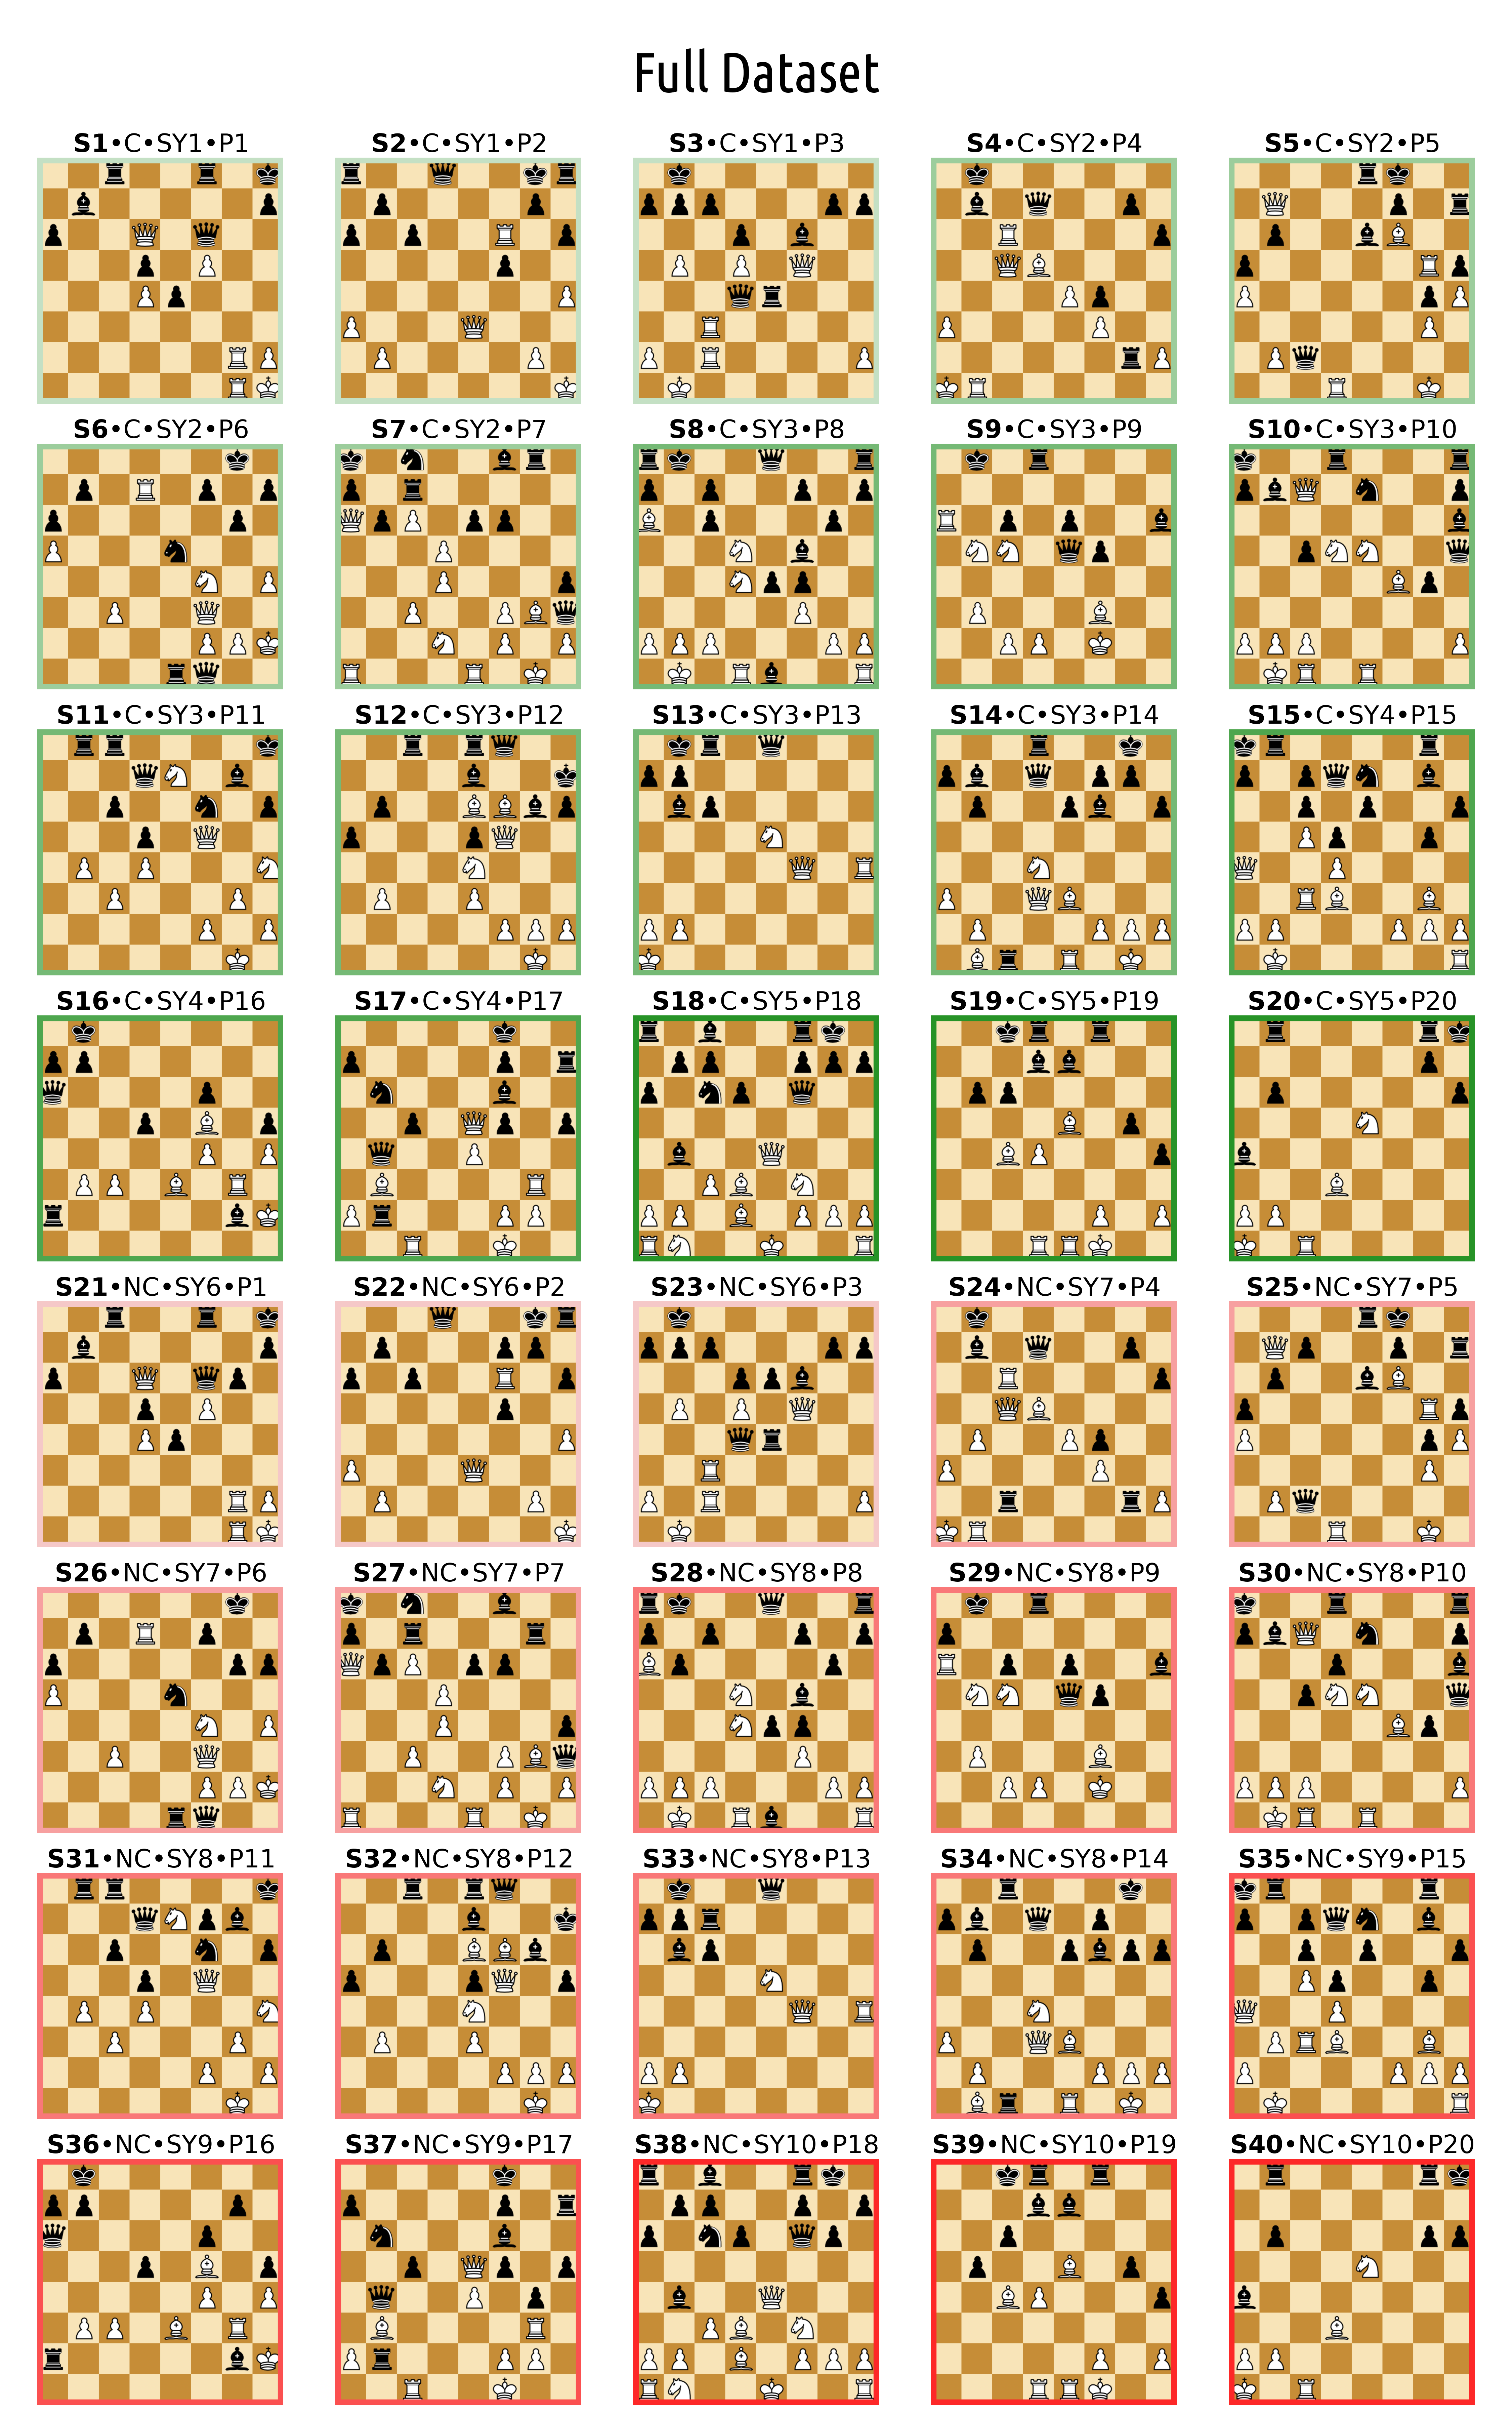
\includegraphics[width=0.8\linewidth]{write/figures/stimuli_with_tags.png}
  \caption{\textbf{Full stimulus set used in the experiment.} Each chessboard represents a unique stimulus from the dataset. The label above each board encodes: \textbf{S} (stimulus number), \textbf{C} or \textbf{NC} for checkmate and non-checkmate respectively, \textbf{SY} (strategy index), and \textbf{P} (visual pair). Borders are shaded: green tones for checkmate boards, red tones for non-checkmates. The hue intensity corresponds to the underlying strategy type.}
  \label{suppfig:all_stims}
\end{figure}

\supplementarysection{Stimulus Set Details}\label{suppsec:all_stims}

This supplementary section provides a comprehensive overview of the 40 chessboard stimuli used in the experiment, each labeled and visualized in Supplementary Fig.~\ref{suppfig:all_stims} and reported in Supplementary Table~\ref{supptab:stim_fens}. Stimuli were constructed to systematically vary along three key dimensions: whether they depicted an imminent checkmate (Checkmate vs.\ Non-checkmate), the tactical strategy leading to the checkmate (Strategy Type), and perceptual similarity (Visual Pairing). 

\emph{Checkmate} boards (C/NC) depicted configurations in which a forced mate sequence for White against Black existed, resolvable in four or fewer moves. Each checkmate board (denoted ``C'' in the figure) was paired with a non-checkmate counterpart (``NC'') that preserved the overall structure and piece configuration but introduced a minimal intervention—typically the repositioning of a single pawn—to neutralize the mating sequence while maintaining close visual similarity.

\emph{Strategy types} (SY) were defined according to both piece involvement and underlying tactical features, reflecting qualitative distinctions in how mating sequences are structured. These include queen–rook combinations (SY1 and SY6), involving coordinated linear tactics; supported attacks with minor pieces (SY2 and SY7), where auxiliary knights or bishops play a crucial role in sustaining the queen mate; minor piece mating nets (SY3 and SY8), relying on spatial confinement by knights and bishops; bishop-driven forcing moves (SY4 and SY9), emphasizing long-range control; and one-move checkmates (SY5 and SY10), which require minimal calculation and serve as structurally simple baselines.

\emph{Visual pairing} (P) designates stimuli matched primarily for perceptual similarity while holding relational structure constant. For each position, we also recorded the total number of pieces, the count of legal moves, the side of the board occupied by the defending king (left = 0, right = 1), and the dominant tactical motif characterizing the checkmate sequence. Where applicable, the number of moves required to reach checkmate is also noted.

\supplementarysection{fMRI data pre-processing}\label{suppsec:fmri-preproc}
\textbf{Anatomical data preprocessing} 
A total of 1 T1-weighted (T1w) images was found within the input BIDS dataset per subject. The T1w image was corrected for intensity non-uniformity (INU) with \texttt{N4BiasFieldCorrection} \cite{n4}, distributed with ANTs 2.5.1 \cite[RRID:SCR\_004757]{ants}, and used as T1w-reference throughout the workflow. The T1w-reference was then skull-stripped with a \emph{Nipype} implementation of the \texttt{antsBrainExtraction.sh} workflow (from ANTs), using OASIS30ANTs as target template. Brain tissue segmentation of cerebrospinal fluid (CSF), white-matter (WM) and gray-matter (GM) was performed on the brain-extracted T1w using \texttt{fast} \cite{fsl_fast} (RRID:SCR\_002823). Brain surfaces were reconstructed using \texttt{recon-all} \cite[FreeSurfer 7.3.2, RRID:SCR\_001847,][]{fs_reconall}, and the brain mask estimated previously was refined with a custom variation of the method to reconcile ANTs-derived and FreeSurfer-derived segmentations of the cortical gray-matter of Mindboggle \cite[RRID:SCR\_002438,][]{mindboggle}. Volume-based spatial normalization to one standard space (MNI152NLin2009cAsym) was performed through nonlinear registration with \texttt{antsRegistration} (ANTs 2.5.1), using brain-extracted versions of both T1w reference and the T1w template. The following template was selected for spatial normalization and accessed with \emph{TemplateFlow}
\cite[24.2.0,][]{templateflow}: \emph{ICBM 152 Nonlinear Asymmetrical template version 2009c} \cite{mni152nlin2009casym} (RRID:SCR\_008796; TemplateFlow ID: \texttt{MNI152NLin2009cAsym}).

\textbf{Functional data preprocessing}
For each of the BOLD runs found per subject, the following preprocessing was performed. First, a reference volume was generated, using a custom methodology of \emph{fMRIPrep}, for use in head motion correction. Head-motion parameters with respect to the BOLD reference (transformation matrices, and six corresponding rotation and translation parameters) are estimated before any spatiotemporal filtering using \texttt{mcflirt} \cite{mcflirt}. The BOLD reference was then co-registered to the T1w reference using \texttt{bbregister} (FreeSurfer) which implements boundary-based registration \cite{bbr}. Co-registration was configured with six degrees of freedom. Several confounding time-series were calculated based on the \emph{preprocessed BOLD}: framewise displacement (FD), DVARS and three region-wise global signals. FD was computed using two formulations following Power (absolute sum of relative motions, \cite{power_fd_dvars}) and Jenkinson (relative root mean square displacement between affines, \cite{mcflirt}). FD and DVARS are calculated for each functional run, both using their implementations in \emph{Nipype} following the definitions by \cite{power_fd_dvars}. The three global signals are extracted within the CSF, the WM, and the whole-brain masks. Additionally, a set of physiological regressors were extracted to allow for component-based noise correction \emph{CompCor} \cite{compcor}. Principal components are estimated after high-pass filtering the \emph{preprocessed BOLD} time-series (using a discrete cosine filter with 128s cut-off) for the two \emph{CompCor} variants: temporal (tCompCor) and anatomical (aCompCor). tCompCor components are then calculated from the top 2\% variable voxels within the brain mask. For aCompCor, three probabilistic masks (CSF, WM and combined CSF+WM) are generated in anatomical space. The implementation differs from that of Behzadi et al.~in that instead of eroding the masks by 2 pixels on BOLD space, a mask of pixels that likely contain a volume fraction of GM is subtracted from the aCompCor masks. This mask is obtained by dilating a GM mask extracted from the FreeSurfer's \emph{aseg} segmentation, and it ensures components are not extracted from voxels containing a minimal fraction of GM. Finally, these masks are resampled into BOLD space and binarized by thresholding at 0.99 (as in the original implementation). Components are also calculated separately within the WM and CSF masks. For each CompCor decomposition, the \emph{k} components with the largest singular values are retained, such that the retained components' time series are sufficient to explain 50 percent of variance across the nuisance mask (CSF, WM, combined, or temporal). The remaining components are dropped from consideration. The head-motion estimates calculated in the correction step were also placed within the corresponding confounds file. The confound time series derived from head motion estimates and global signals were expanded with the inclusion of temporal derivatives and quadratic terms for each \cite{confounds_satterthwaite_2013}. Frames that exceeded a threshold of 0.5 mm FD or 1.5 standardized DVARS were annotated as motion outliers. Additional nuisance timeseries are calculated by means of principal components analysis of the signal found within a thin band (\emph{crown}) of voxels around the edge of the brain, as proposed by \cite{patriat_improved_2017}. The BOLD time-series were resampled onto the following surfaces (FreeSurfer reconstruction nomenclature): \emph{fsnative}. All resamplings were performed with \emph{a single interpolation step} by composing all the pertinent transformations (i.e.~head-motion transform matrices, susceptibility distortion correction when available, and co-registrations to anatomical and output spaces). Gridded (volumetric) resamplings were performed using \texttt{nitransforms}, configured with cubic B-spline interpolation. Non-gridded (surface) resamplings were performed using \texttt{mri\_vol2surf} (FreeSurfer).

Many internal operations of \emph{fMRIPrep} use \emph{Nilearn} 0.10.4 \cite{nilearn} (RRID:SCR\_001362) , mostly within the functional processing workflow. For more details of the pipeline, see \href{https://fmriprep.readthedocs.io/en/latest/workflows.html}{the section corresponding to workflows in \emph{fMRIPrep}'s documentation}. 

\supplementarysection{Split-half Reliability of Behavioral RDMs}\label{suppsec:splithalf_bh_rdm}

To assess the reliability of behavioral Representational Dissimilarity Matrices (RDMs) in Experts and Novices, we computed split-half correlations using a permutation-based approach. For each group (Experts and Novices), we randomly split participants into two non-overlapping halves and compute separate RDMs with the same method as described in Sec.~\ref{sec:bh_rsa_section}. Spearman correlations were then computed between the lower triangles of the two RDMs. This procedure was repeated across 1,000 random permutations, yielding a distribution of split-half correlation coefficients for each group.

To test whether these reliability estimates were significantly greater than zero, we conducted one-sample \textit{t}-tests across the 1,000 permutations for each group. Additionally, we computed split-half correlations \textit{between} groups by comparing random halves of Experts to random halves of Novices, also across 1,000 permutations. Independent-samples \textit{t}-tests were used to compare Experts and Novices on both within- and between-group reliability scores. All statistical tests were two-tailed. All results are reported in Supplementary Table~\ref{supptab:bh_splithalf}.

We found that behavioral RDM reliability was higher in Experts: the mean split-half Spearman correlation \emph{within} the expert group was $r = 0.104$, while Novices showed $r = 0.030$. Split-half correlations \emph{between} Experts and Novices were negative (mean $r = -0.013$), indicating low cross-group similarity. These patterns suggest that expertise is associated with a more stable and shared representational geometry of the task domain: Experts exhibit more consistent pairwise dissimilarity structure across individuals, whereas Novices show weaker and more idiosyncratic structure; the near-zero difference in cross-group correlations ($\Delta r \approx 0$) further implies that expert and novice representations are organized differently rather than reflecting a simple strengthening of a common layout.

\begin{figure}[!htp]
  \centering
  \includegraphics[width=1\linewidth]{write/figures/roi_analysis_univ.png}
  \caption{\textbf{Univariate ROI differences (Experts vs. Novices).} Cortical parcels from the 180-area Glasser atlas showing group differences in second-level GLM contrast maps (\emph{Checkmate} $>$ \emph{Non-checkmate}, \emph{All} $>$ \emph{Rest}). Colors indicate the direction and relative magnitude of the Experts$-$Novices difference in contrast values. Maps are derived from the univariate analyses in Sec.~\ref{sec:fmri_glm}.}
  \label{suppfig:roi_analysis_univ}
\end{figure}

\begin{figure}[!htp]
  \centering
  \includegraphics[width=1\linewidth]{write/figures/roi_analysis_rsa.png}
  \caption{\textbf{ROI summaries of searchlight RSA group differences.} For each model RDM (Checkmate, Strategy, Visual similarity), whole-brain searchlight RSA maps were averaged within Glasser ROIs to compare Experts and Novices. \emph{Left}: uncorrected visualization. \emph{Right}: parcels surviving multiple-comparisons correction. Colors indicate the direction and relative magnitude of the Experts$-$Novices difference in model–brain correspondence. Maps are derived from the RSA analyses in Sec.~\ref{sec:fmri_rsa}.}
  \label{suppfig:roi_analysis_rsa}
\end{figure}

\supplementarysection{ROI analysis from uni and multivariate brain maps}\label{suppsec:roi_analysis}

To identify finer-grained anatomical regions showing significant differences in mean activation between Experts and Novices, we performed an exploratory second-level ROI analysis using the 180-region version of the Glasser parcellation described in Sec.~\ref{sec:rois}. We conducted this analysis on two sets of brain maps: the univariate first-level GLM contrast maps (Sec.~\ref{sec:fmri_glm}), and the searchlight RSA maps from Sec.~\ref{sec:fmri_rsa}. 

To facilitate anatomical interpretation, each ROI was additionally assigned a secondary label from the Harvard–Oxford cortical atlas. This was done by computing the center of mass of each ROI in MNI space and mapping the resulting coordinate to the nearest non-zero voxel in the 2\,mm Harvard–Oxford atlas (thresholded at 25\%). This combined approach allowed us to combine the spatial specificity of the Glasser atlas, which allows for more precise estimates of local activation patterns, with the broader and more familiar anatomical nomenclature of the Harvard-Oxford atlas.

\emph{Univariate contrast maps}
For each participant and contrast (\emph{Checkmate $>$ Non-checkmate}, \emph{All $>$ Rest}), we imported the first-level contrast images and extracted mean signal values from each of the 180 cortical ROIs using the \texttt{NiftiLabelsMasker} implementation in \texttt{nilearn}. This yielded a single scalar value per ROI per participant, resulting in group-level matrices for Experts and Novices that were used for statistical comparison. For each ROI, we performed an independent-samples $t$-test comparing Experts and Novices, and computed the mean group difference, $t$-statistic, FDR-corrected $p$-value, and the 95\% confidence interval of the difference. Results for significant ROIs are reported in Supplementary Table~\ref{supptab:roi_analysis_univ_allrest} and visualized in Supplementary Figure \ref{suppfig:roi_analysis_univ}.

Univariate analyses were suggestive of several activation spots at or near locations that have been previously investigated in expertise literature, but in many cases these differences did not survive correction for multiple comparisons. This strengthens the suspicion that was the major motivation for our study: namely, that the classic univariate approach is not sensitive to the many ways in which expertise changes neural processing.

\emph{RSA searchlight maps}
To facilitate anatomical interpretation of the searchlight RSA results, and to complement the univariate group-level analysis with a "content-oriented" approach, we applied the same second-level ROI-based procedure described in the above paragraph. For each participant theoretical model (Checkmate, Strategy, Visual Similarity), we imported the individual whole-brain correlation maps obtained from the searchlight (see Sec.~\ref{sec:neurosynth_analysis}), extracted the mean correlation value within each of the 180 Glasser ROIs, and performed independent-samples $t$-tests comparing Experts and Novices ROI-wise. Anatomical labels from the Harvard–Oxford cortical atlas were assigned to each ROI based on their center of mass.

Results from this analysis (see Supplementary Tables~\ref{supptab:roi_analysis_rsa_check} and \ref{supptab:roi_analysis_rsa_strategy}, and Supplementary Figure \ref{suppfig:roi_analysis_rsa}) showed more extensive networks involved in chess expertise than the univariate counterpart. On the one hand, this suggests that multi-variate approaches may tap onto complementary aspects than univariate ones, and on the other that expertise effects in the brain may involve broader networks than previously thought.

\begin{figure}[!htp]
  \centering
  \includegraphics[width=1\linewidth]{write/figures/rsa_vs_decoding_main.png}
    \caption{\textbf{Comparison of RSA and decoding on the main model dimensions.} ROI-wise summaries of model–brain correspondence (RSA) versus linear classification accuracy (SVM decoding) for the three primary dimensions (Checkmate, Strategy, Visual similarity). Panels juxtapose RSA (left) and decoding (right) to highlight convergences and divergences across the 22 Glasser ROIs. Colors indicate ROI groups; asterisks indicate significant regions (Experts $>$ Novices) after FDR correction.}
      \label{suppfig:rsa_vs_decoding_main}
\end{figure}

\begin{figure}[!htp]
  \centering
  \includegraphics[width=1\linewidth]{write/figures/rsa_vs_decoding.png}
    \caption{\textbf{Comparison of RSA and decoding on finer dimensions (checkmate stimuli only).} As in Fig.~\ref{suppfig:rsa_vs_decoding_main}, but restricted to checkmate boards and extended to finer categorizations (Strategy within checkmates, Motif, Total pieces, Legal moves, and White moves to mate). RDMs derived from the finer dimensions are shown in the central panel. Colors indicate ROI groups; asterisks indicate significant regions (Experts $>$ Novices) after FDR correction.}
      \label{suppfig:rsa_vs_decoding_finer}
\end{figure}

\supplementarysection{Brain Decoding}\label{suppsec:brain-decoding}
% Purpose and rationale
To assess whether local voxel patterns encoded linearly decodable information about chess-relevant categories, we conducted multivariate classification analyses using support vector machines (SVMs). These analyses evaluated the discriminability of activation patterns across different conditions within each region of interest (ROI), providing a functional readout of category-selective information.

% Input data and ROI setup
Classification analyses were implemented in MATLAB R2024b using the CoSMoMVPA toolbox \cite{oosterhof2016cosmomvpa}. As explained in Sec.~\ref{sec:fmri_glm}), we used the unsmoothed beta estimates of the 40 conditions as the input of these analyses. For each subject and run, multi-voxel patterns were extracted from predefined ROIs, including bilateral cortical mask from the Glasser atlas~\cite{glasser2016multi} (See section \ref{sec:rois} for more details). All analyses were performed separately for each ROI and participant.

% SVM training, partitioning, and targets
For each ROI, a linear SVM classifier (\texttt{@cosmo\_classify\_svm}) was trained to discriminate between condition labels derived from the experimental design. Classification targets were constructed from categorical regressors (e.g., Checkmate, Strategy, Visual similarity). The data were partitioned using an $n$-fold cross-validation scheme across runs (leave-one-run-out), with balanced folds ensured via \texttt{cosmo\_balance\_partitions}. Within each fold, voxel patterns were labeled with their corresponding class and used to train and test the classifier.

% Accuracy computation and filtering
Decoding accuracy was defined as the mean classification performance across cross-validation folds. ROIs with fewer than 10 usable voxels were excluded to ensure minimum feature dimensionality. Accuracy scores were computed independently for each participant, regressor, and ROI.

% Intro and visual similarity (no robust results)
Supplementary Table~\ref{tab:svm_roi_summary} and Supplementary Fig.~\ref{suppfig:rsa_vs_decoding_main} reports SVM decoding accuracy across ROIs for each main model dimension. Decoding based on the \emph{Visual Similarity} model yielded restricted but significant effects. While some ROIs showed above-chance classification (e.g., posterior cingulate: $M = 0.028$; superior parietal: $M = 0.028$), the majority of visual and high-level areas did not exhibit significant decoding for this perceptual dimension. Decoding accuracy in early and primary visual cortex was low and non-significant (e.g., early visual: $M = -0.040$), suggesting that visual similarity alone did not strongly shape the separability of neural patterns in these regions.

% Strategy decoding: broad, robust, parietal-frontal + dorsal stream
In contrast, decoding of the \emph{Strategy} dimension revealed robust group-level accuracy across a broad network of ROIs. Experts showed reliable above-chance decoding in the superior parietal lobule ($M = 0.046$), inferior parietal lobule ($M = 0.035$), and dorso-lateral prefrontal cortex ($M = 0.027$). Additional significant decoding was observed in premotor cortex ($M = 0.033$), paracentral lobule and mid-cingulate ($M = 0.024$), and insular and frontal opercular cortex ($M = 0.013$). Effects also extended to dorsal stream visual areas ($M = 0.018$), highlighting their role in abstract relational processing. These findings indicate that expert representations are sufficiently structured along strategy-related dimensions to permit reliable linear classification.

% Checkmate decoding: similar pattern, high-level areas
Decoding of \emph{Checkmate vs. Non-checkmate} boards yielded a similar spatial profile. High classification accuracy was observed in dorso-lateral prefrontal cortex ($M = 0.080$), inferior parietal cortex ($M = 0.089$), and superior parietal cortex ($M = 0.053$). Additional significant effects were found in lateral temporal cortex ($M = 0.052$), premotor areas ($M = 0.052$), and posterior cingulate cortex ($M = 0.035$), indicating that goal-related distinctions such as checkmate status were reliably encoded in higher-order associative cortices.

% Finer decoding
Aside our main decoding analysis (i.e., on the three main dimension built into our dataset), we also performed a finer decoding analysis on five additional possible categorizations of the checkmate boards. This finer analysis allow us to assess what information can be decoded within the checkmate class, offering a proxy into how strategic information may be structured. Specifically, we performed a decoding analysis on: Strategy (the same as in the main analysis, but now using only the 20 checkmate chess boards), Motif, Total number of pieces, Total number of available legal moves, and Number of white moves to checkmate. All the results for this analysis (and their RSA counterparts) are reported in Supplementary Tables~\ref{tab:svm_roi_summary_checkonly} and~\ref{tab:rsa_roi_summary_checkonly}, and visualized in Supplementary Fig.~\ref{suppfig:rsa_vs_decoding_finer}.

\begin{figure}[!htp]
  \centering
  \includegraphics[width=1\linewidth]{write/figures/rdm_intercorr.png}
    \caption{\textbf{Orthogonality of representational dissimilarity matrices.} 
    \textbf{Top row:} Bar plots showing the Spearman correlation between each target RDM and the other two predictors, both as pairwise correlations and partial correlations (controlling for the third RDM). Each bar reflects the strength of association ($\rho$), with partial correlations labeled as ``(partial X)'' to indicate the variable that was controlled for. 
    \textbf{Bottom row:} Variance partitioning results for each target RDM. Bars indicate the proportion of variance uniquely explained by each predictor RDM, variance shared between predictors, and residual (unexplained) variance. Larger unique and smaller shared contributions suggest greater orthogonality among representational structures.}
      \label{suppfig:rdm_orthogonality}
\end{figure}

\supplementarysection{Orthogonality Across RDMs}

To quantify the degree of overlap and separability among representational structures in our dataset, we first computed pairwise Spearman correlations between the flattened upper triangle of each model RDM (excluding the diagonal), providing a measure of shared variance in representational structure. We then computed partial Spearman correlations, which estimate the relationship between two RDMs while controlling for variance explained by the third. For instance, the partial correlation between the Checkmate and Strategy RDMs, controlling for Visual Similarity, reflects their unique association independent of the shared structure with the Visual RDM. 

To further disentangle representational overlap, we further conducted a variance partitioning analysis based on nested linear regression models. Each RDM was treated in turn as a dependent variable, with the remaining two serving as predictors. We fit a full multiple linear model using both predictors to explain variance in the target RDM, and two reduced models each omitting one predictor. The unique variance explained by each predictor was calculated as the difference in $R^2$ between the full model and the corresponding reduced model. Shared variance was defined as the portion of $R^2$ explained by both predictors jointly, beyond their individual contributions, and residual variance captured the unexplained portion.
Formally, given a target RDM $Y$ and two predictors $X_1$ and $X_2$, we define:
\[
\begin{aligned}
R^2_{\text{full}} &= R^2(Y \sim X_1 + X_2) \\
R^2_{\text{reduced}_1} &= R^2(Y \sim X_2) \\
R^2_{\text{reduced}_2} &= R^2(Y \sim X_1) \\
\text{Unique}_{X_1} &= R^2_{\text{full}} - R^2_{\text{reduced}_1} \\
\text{Unique}_{X_2} &= R^2_{\text{full}} - R^2_{\text{reduced}_2} \\
\text{Shared} &= R^2_{\text{full}} - \text{Unique}_{X_1} - \text{Unique}_{X_2} \\
\text{Residual} &= 1 - R^2_{\text{full}}
\end{aligned}
\]
Any negative values arising from this decomposition due to noise or multicollinearity were set to zero for interpretability. This approach provides a formal quantification of the unique and shared variance attributable to each representational model, allowing us to assess the degree of orthogonality between theoretical representational geometries.

The variance partitioning analysis revealed that the three RDMs are well-separated and largely independent (see~\ref{suppfig:rdm_orthogonality}, with each predictor explaining predominantly unique rather than shared variance. This orthogonality validates the theoretical distinctiveness of the representational structures captured by the \textit{Check}, \textit{Strategy}, and \textit{Visual} RDMs, indicating that they reflect genuinely different aspects of chess board representation. The predominance of unique variance over shared variance supports the use of these RDMs as independent predictors in subsequent analyses, as they capture complementary rather than redundant information about stimulus similarity structure.

\begin{figure}[!htp]
 \centering
 \includegraphics[width=0.6\linewidth]{write/figures/eyetrack.png}
   \caption{\textbf{Decoding chess expertise from eye-tracking data.} Each dot represents the cross-validated accuracy from one of the $k=20$ stratified group folds. \textbf{Left:} decoding based on two-dimensional gaze coordinates (x, y). \textbf{Right:} decoding based on displacement from screen center. The solid horizontal line shows the mean accuracy across folds; the dashed line indicates chance level (0.5). The shaded band marks the 95\% confidence interval around the mean, computed using the Student's $t$-distribution.}
 \label{suppfig:eyetrack_results}
\end{figure}

\supplementarysection{Groups cannot be inferred from estimated eye-movements}

To investigate whether estimated eye-movement patterns differ systematically between chess Experts and Novices, we performed two separate decoding analyses using support vector machines (SVM). The first analysis used the estimated gaze coordinates (x, y), while the second used the corresponding displacements from the center of the screen. These estimates were derived from functional MRI data using BidsMReye (\href{https://github.com/cpp-lln-lab/bidsMReye}), a BIDS-ready version of DeepMReye~\cite{frey2021magnetic}.

We included the full sample of 40 participants (20 Experts and 20 Novices). For each participant, all available task runs were used; each run was treated as an independent sample. The input features for each sample were constructed by flattening the time series of the gaze coordinates or displacement values within a run, resulting in a subject-run-level feature vector. This yielded a feature matrix $X \in \mathbb{R}^{n \times d}$, where $n$ is the number of runs and $d$ is the number of timepoints times two (for x and y) or one (for displacement). Binary class labels $y \in \{0, 1\}^n$ indicated expertise (expert = 1, novice = 0), and subject identifiers were recorded to define cross-validation groups.

We assessed classification performance using stratified group $k$-fold cross-validation with $k = 20$ folds, as implemented in \texttt{StratifiedGroupKFold} from \texttt{scikit-learn}. This procedure ensured that samples from the same participant were never split between training and test sets (i.e., we used 19 subjects per group as training set and one subject per group as test set). Folds were stratified by class to preserve expert/novice balance.

Within each fold, we trained a support vector classifier with a linear kernel using a pipeline that included z-scoring of input features via \texttt{StandardScaler}. The model was trained on all runs from all training participants and evaluated on the runs from the held-out participants. For each test sample, we recorded the predicted class label and the posterior probability (decision function output) for being classified as an expert. This process was repeated for all folds, and the predicted labels and probabilities were aggregated across folds.

Performance was quantified using overall accuracy, balanced accuracy, and F1-score. To statistically assess whether decoding exceeded chance, we performed a one-sample $t$-test on the distribution of fold-wise accuracies against a null hypothesis of 0.5 (chance), and computed the binomial probability of the number of correctly classified runs under chance performance. Results are reported in Supplementary Fig. \ref{suppfig:eyetrack_results} and Supplementary Table \ref{supptab:et_decoding_results}.

\begin{figure}[!ht]
    \centering
    \includegraphics[width=1\linewidth]{write/figures/pr_supp.png}
    \caption{\textbf{Relationship between PR and ROI size} (number of voxels), plotted separately for Experts (left), Novices (center), and group differences (right). Each dot represents one ROI; lines indicate linear regression fits, with corresponding Pearson correlation coefficients. These analyses test whether PR scales with anatomical extent and whether this relationship differs between groups.
  }
    \label{suppfig:pr_suppl}
\end{figure}

\supplementarysection{Participation ratio is not predicted by ROI size}

To assess how regional dimensionality relates to anatomical size, we computed the participation ratio (PR) within each cortical ROI for each participant. We then averaged PR values across participants within each group (Experts and Non-Experts) and calculated the difference (Expert minus Non-Expert) per ROI. Finally, we visualized and quantified the relationship between PR and ROI size by plotting these measures against each other and computing Pearson correlation coefficients (see Fig.~\ref{suppfig:pr_suppl}).

\begin{figure}[!htp]
    \centering
    \includegraphics[width=.8\linewidth]{write/figures/terms_flat.png}
    \caption{\textbf{Neurosynth meta-analytic cognitive maps.} The maps are showed in volume space along with the corresponding surface projection.}
    \label{suppfig:flat_terms}
\end{figure}

\clearpage

\input{write/tables/stimuli}
\input{write/tables/bh_rdm_splithalf}
\input{write/tables/rsa_main_dims}
\input{write/tables/decoding_main_dims}
\input{write/tables/mvpa_extended_dimensions}
\input{write/tables/pr_ttest}
\input{write/tables/neurosynth_rsa}
\input{write/tables/neurosynth_univ}
\input{write/tables/roi_maps_rsa} 
\input{write/tables/roi_maps_univ} 
\input{write/tables/et_decoding}

